\chapter{Extending Classes}

Two important concepts in object-oriented programming are {\em composition} and {\em inheritance}. In {\em Think Java, 2nd Edition}, you have seen composition in Chapter 13 and inheritance in Chapter 14, but mostly by example. We're going to go into more detail on both of these concepts here.

\section{Composition}
\index{composition}
\index{aggregating class}
\index{aggregated class}
\index{class!aggregating}
\index{class!aggregated}

Composition happens when an object is made up of other objects. We saw this in Chapter 13, where a \java{Deck} was made up of an array of \java{Card} objects:

\begin{code}
public class Deck {
    private Card[] cards; 
    ...
}
\end{code}

Composition is also known as a {\em Has-A} relationship.  (A \java{Deck} {\em has an} array of \java{Card}s).  Put formally, the \java{Deck} is the {\em aggregating class}, and the \java{Card} class is is the {\em aggregated class}.

When we draw a UML diagram involving composition, as in Figure~\ref{fig.aggregation}, we use an arrow with a diamond head to indicate aggregation, and we can also add notation here that shows that one \java{Deck} contains many \java{Card} objects.

\begin{figure}[!ht]
\begin{center}
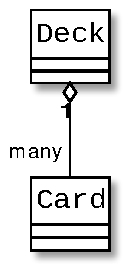
\includegraphics[scale=0.75]{figs/ch14/aggregation.pdf}
\caption{UML Diagram Showing Aggregation - a Deck has Card(s)}
\label{fig.aggregation}
\end{center}
\end{figure}

Let's use composition to build a Java simulation of a toaster. What things is a toaster built from?

\begin{itemize}
\item A chassis with a number of slots (at least one, at most four)
\item A lever to push bread down or pop it out
\item A power supply to turn the toaster on and off
\item A dial to control the darkness (1=light, 10=dark)
\end{itemize}

The first two of these are built by the toaster company. But the company that makes toasters doesn't build the power supply or the dial (which has circuitry to control the current flow). Instead, those are parts they order from some other companies and put into the chassis.

That means that our \java{Toaster} {\em has-a} \java{PowerSupply} object and {\em has-a} \java{Dial} object. Figure~\ref{fig.toasterComposition} shows the UML diagram. You can see the full code in the file {\em ch14/ToasterTest.java} in the repository.

\begin{figure}[!ht]
\begin{center}
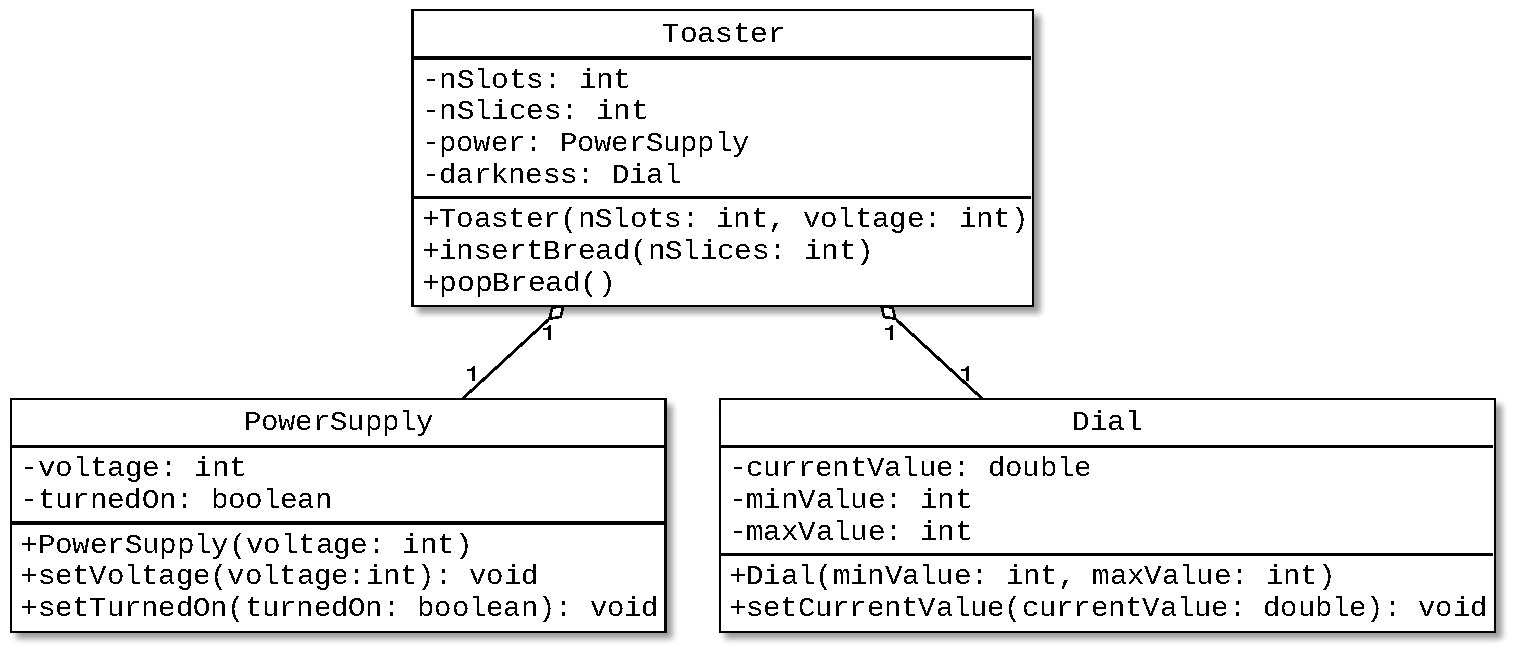
\includegraphics[scale=0.5]{figs/ch14/toaster.pdf}
\caption{UML Diagram Showing a Toaster composed of a PowerSupply and Dial}
\label{fig.toasterComposition}
\end{center}
\end{figure}

Before we see how composition affects the way we construct and manipulate objects, let's give a few more instances of composition ({\em has-a}) relationships. Using composition reflects the way objects are built out of other objects (parts). Each of the sub-parts has its own attributes and things that it can do (its ``methods''). Notice that we sometimes need multiple instances of a sub-part when constructing the larger object.

\begin{itemize}
\item A printer has a power supply, printer drum, and toner cartridge.
\item A bicycle has a gear assembly, handbrakes (2), and tires (2).
\item A refrigerator has a power supply, an icemaker, and a compressor.
\item A window in a word processor has a text area, a ribbon (icons for manipulating text), and two scroll bars (horizontal and vertical).
\end{itemize}

Back to the toaster. Here are constructors for the \java{PowerSupply} and \java{Dial} classes:

\begin{code}
public PowerSupply(int voltage) {
    if (voltage == 220) {
        this.voltage = voltage;
    } else {
        this.voltage = 110;
    }

    // new power supplies are always turned off
    this.turnedOn = false;
}

public Dial(int minValue, int maxValue) {
    this.minValue = minValue;
    this.maxValue = maxValue;
    // new dials are always set to lowest value
    this.dialValue = minValue;
}
\end{code}

Now, look at how the \java{Toaster} class starts, with line numbers for reference:

\begin{code}
 1 class Toaster {
 2     private int nSlots;
 3     private int nSlices;
 4     private PowerSupply power;
 5     private Dial darkness;
 6  
 7     public Toaster(int nSlots, int voltage) {
 8         this.nSlots = Math.max(1, Math.min(4, nSlots));
 9         this.nSlices = 0;
10         this.power = new PowerSupply(voltage);
11         this.darkness = new Dial(1, 10);
12     }
13     // ...
14 }
\end{code}

The constructor in line 7 has two parameters: the number of slots in the toaster and what voltage it should have. The number of slots and number of slices of bread currently in the toaster are attributes belonging to the \java{Toaster} class, and those get set directly.

The power supply is an object, which is why line 10 has to call the \java{PowerSupply} constructor to build a power supply with the desired voltage. Think of this as the toaster company calling up the power supply company and telling them “send me a 110-volt power supply” and putting that power supply into the finished toaster.

Similarly, line 11 has to call the \java{Dial} constructor to build a dial with a range of 1-10.

Although a real-life toaster is composed of parts, all of the controls are on the toaster's exterior. We don't expect---or want---the customer to have to directly access the power supply to turn the toaster on! Similarly, we want to provide methods in the \java{Toaster} class that will give programs that use the class access to the private methods and attributes of \java{power} and \java{darkness}:

\begin{code}
public boolean isTurnedOn() {
    return this.power.isTurnedOn();
}

public void setTurnedOn(boolean turnedOn) {
    this.power.setTurnedOn(turnedOn);
}

public double getDialValue() {
    return this.darkness.getDialValue();
}

public void setDialValue(double dialValue) {
    this.darkness.setDialValue(dialValue);
}
\end{code}

Now we can write a program that creates a \java{Toaster} object and makes it do things:

\begin{code}
public class ToasterTest {
    public static void main(String[] args) {
        Toaster euroFour = new Toaster(4, 220);
       
        euroFour.setTurnedOn(true);
        euroFour.setDialValue(4.5);
        euroFour.insertBread(1);
        
        System.out.println(euroFour);
    }
}
\end{code}

To summarize this discussion of composition:

\begin{itemize}
\item Use composition when you have objects that are built up from other objects.
\item Provide methods in an object to give users access to \java{private} attributes and methods of the sub-objects.
\end{itemize}

\section{Inheritance}
An {\em Is\-A} relationship is known as {\em inheritance}. For example, a \java{Hand} class (subclass) also {\em is-a} \java{CardCollection} class (superclass). In Java, we use \java{extends} to indicate inheritance:

\begin{code}
public class Hand extends CardCollection {
   ...
}
\end{code}

Figure~\ref{fig.simpleInheritance} shows the UML for inheritance, using an open arrowhead:

\begin{figure}[!ht]
\begin{center}
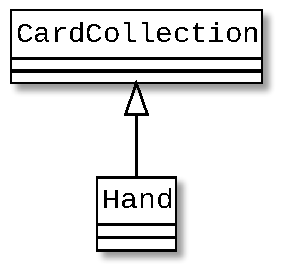
\includegraphics[scale=0.75]{figs/ch14/inheritance.pdf}
\caption{UML Diagram Showing Inheritance - a Hand is a CardCollection}
\label{fig.simpleInheritance}
\end{center}
\end{figure}

Other examples of this sort of relationship:

\begin{itemize}
\item An electric bicycle {\em is a} bicycle (with extra attributes and capabilities)
\item A trumpet {\em is a} bugle with valves (keys) that give the ability to play more notes
\item An alarm clock {\em is a} desk clock with extra attributes and capabilities
\item In a computer application, a ``combo box'' {\em is a} drop-down menu with extra capabilities (you can type the value as well as select it from the list)
\end{itemize}

Without inheritance, we would have to represent the \java{Bicycle} and \java{ElectricBicycle} classes as shown in Figure~\ref{fig.nonInheritedBikes}

\begin{figure}[!ht]
\begin{center}
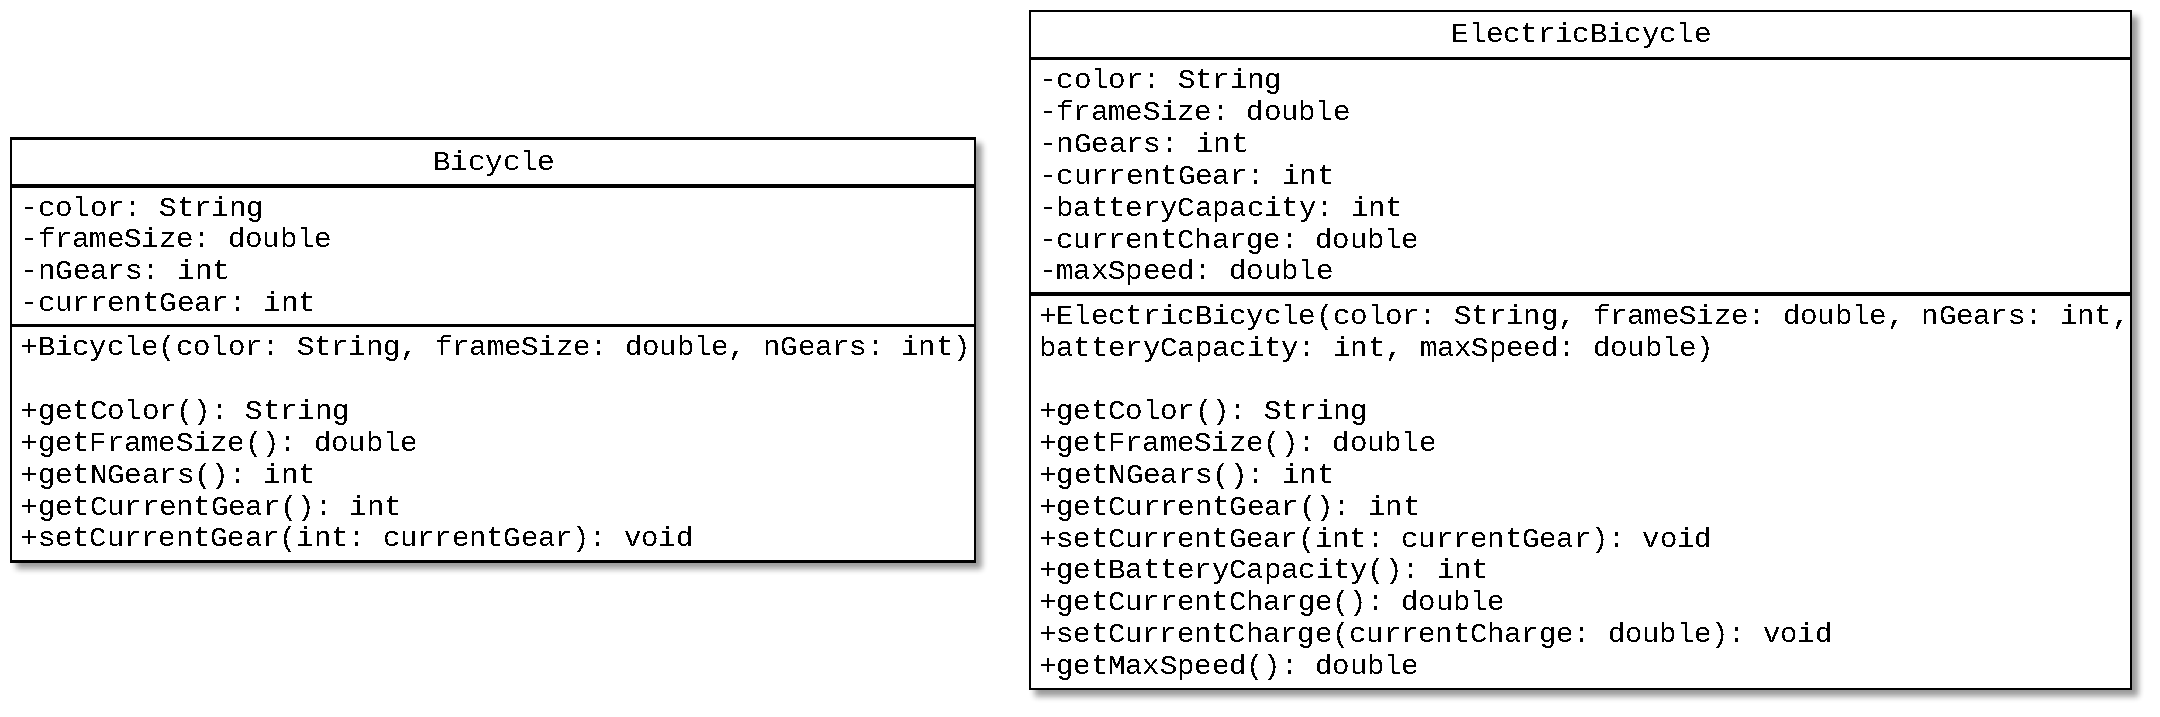
\includegraphics[scale=0.3]{figs/ch14/non_inherited_bikes.pdf}
\caption{UML Diagram of Two Separate Classes for Bicycle and ElectricBicycle}
\label{fig.nonInheritedBikes}
\end{center}
\end{figure}

That's a lot of duplicated code when we translate it to Java. If we say that
\java{ElectricBicycle extends Bicycle}, that means that \java{ElectricBicycle} {\em inherits} all of \java{Bicycle}'s methods and attributes. All we have to include now in \java{ElectricBicycle} are the attributes and methods that add extra capabilities to an electric bicycle, as shown in Figure~\ref{fig.inheritedBikes}

In this example, \java{Bicycle} is called the {\em superclass} or {\em parent class}, and \java{ElectricBicycle} is called the {\em subclass} or {\em child class}.  As in the real world, the child inherits things from the parent.\footnotemark

\footnotetext{With one exception: as the joke says, ``Parents inherit their gray hair from their children.''}

\begin{figure}[!ht]
\begin{center}
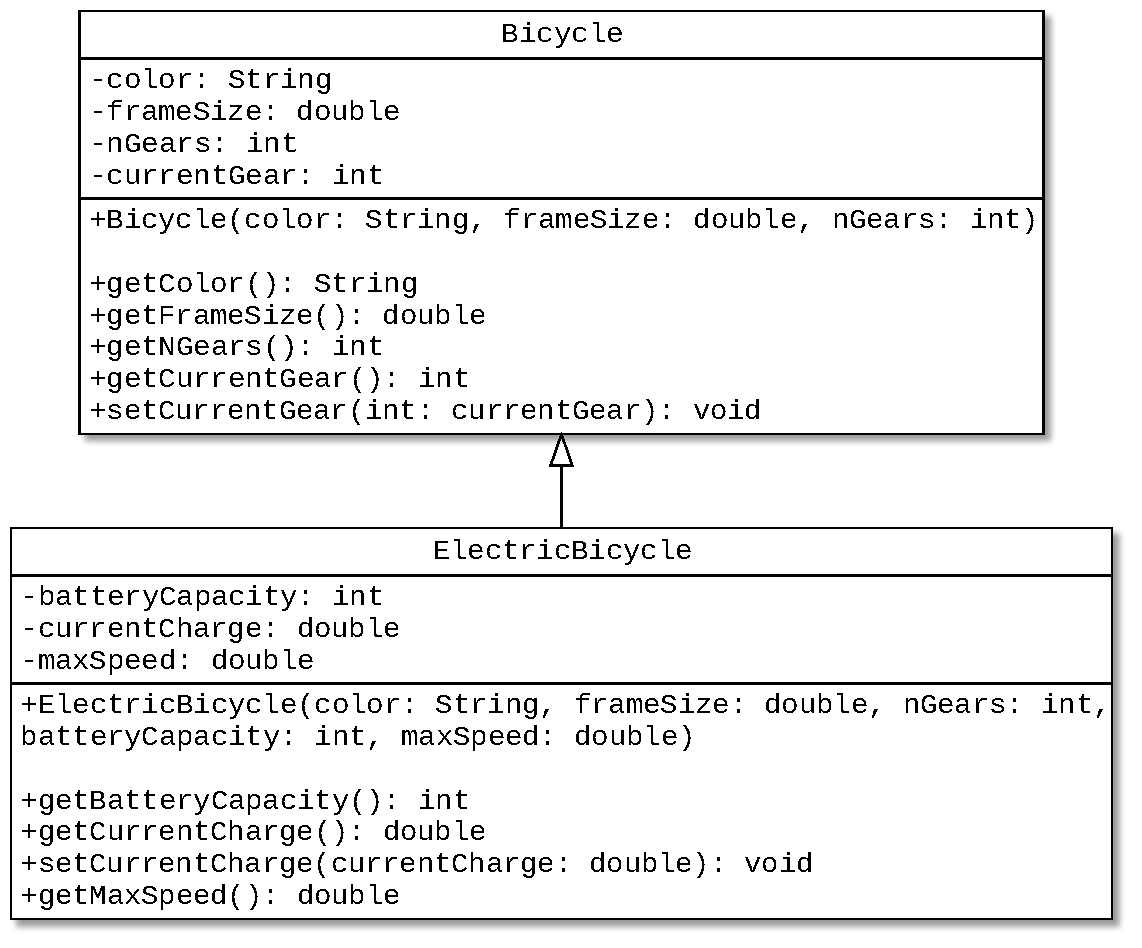
\includegraphics[scale=0.5]{figs/ch14/inherited_bikes.pdf}
\caption{UML Diagram of ElectricBicycle Extending the Bicycle Class}
\label{fig.inheritedBikes}
\end{center}
\end{figure}

Before we go into details about how to use inheritance in Java, let's take a break for a short exercise:

\section{Exercise: Composition vs. Inheritance}

\begin{exercise}
In this exercise, we will explore {\em has-a} and {\em is-a} relationships. First, state whether the relationship of the following classes is composition or inheritance, and draw the UML diagram showing that relationship.

\begin{itemize}
    \item \java{Address} and \java{Student}
    \item \java{Car} and \java{Vehicle}
    \item \java{Account} and \java{SavingsAccount}
    \item \java{State}, \java{Capital}, and \java{Country}
    \item \java{Instructor}, \java{Course}, and \java{Textbook}
    \item \java{Dog}, \java{Cat}, and \java{Animal}
    \item \java{Rectangle}, \java{Circle}, \java{Square}, and \java{Shape}
\end{itemize}

For classes that exhibit the inheritance relationship, could you name a few data fields/attributes for the superclass? Could you name a few for the subclass only?

For example, \java{Teacher} (subclass) is also a \java{Person} (superclass). 
Data fields for \java{Person} are: name, age, address, etc.
Data fields for \java{Teacher} are: school, hire date etc.

\end{exercise}

\section{Inheritance (continued)}

Let's use a smaller example for our continued discussion of inheritance.  We'll have an \java{Item} class, which represents an item in a store. An \java{Item} instance has a name, a SKU (stock keeping unit), and a price. This is the parent class. We also have a \java{SaleItem} class, which is a child class. In addition to a name, SKU, and price (which it inherits from the parent class), a \java{SaleItem} has a discount percentage (expressed as a decimal). Figure~\ref{fig.itemObject} shows the UML diagram for these two classes:

\begin{figure}[!ht]
\begin{center}
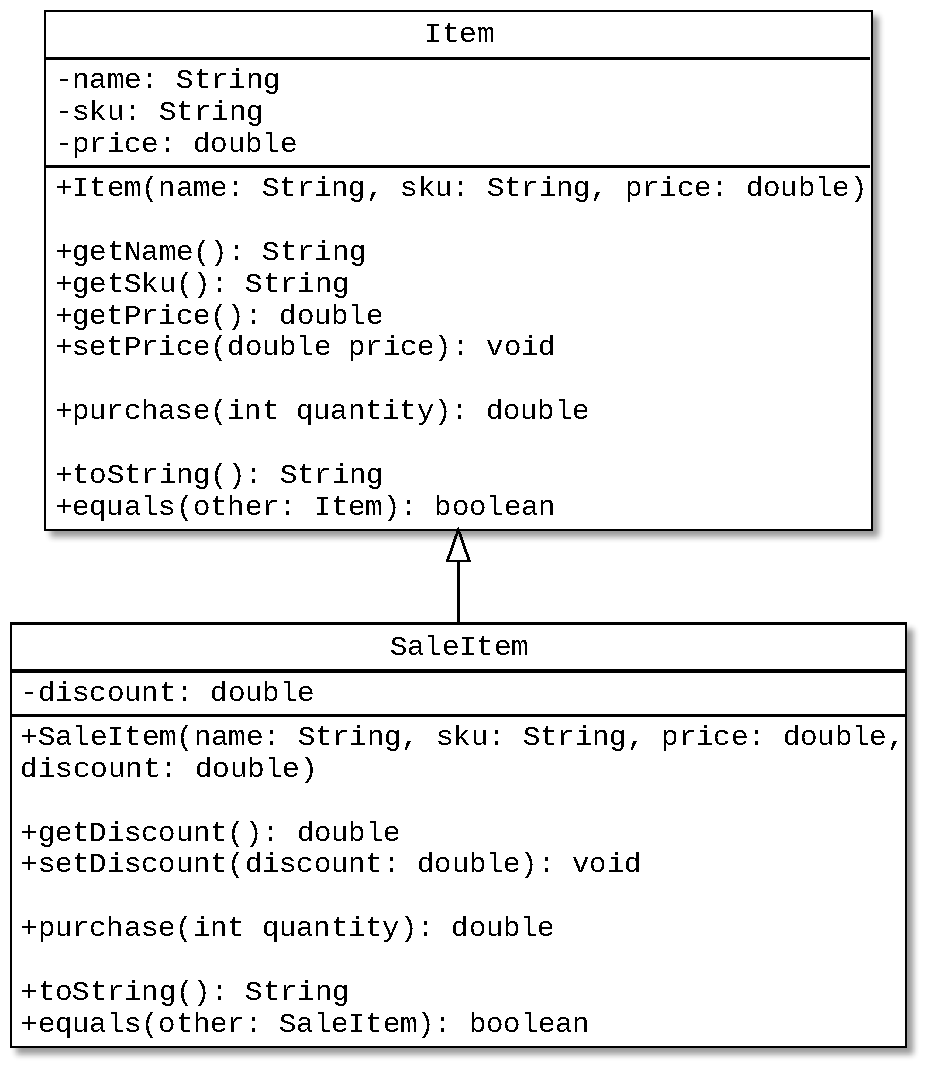
\includegraphics[scale=0.5]{figs/ch14/item.pdf}
\caption{UML Diagram of Item and SaleItem classes}
\label{fig.itemObject}
\end{center}
\end{figure}

There are no setters for the \java{name} and \java{sku} attributes; once an item is created, those attributes should never change.

Here is the code for \java{Item}, which you will find in the repository in file {\em ch14/Item.java}:

\begin{code}
public class Item {
    private String name;
    private String sku;
    private double price;
    
    public Item(String name, String sku, double price)  {
        this.name = name;
        this.sku = sku;
        this.price = Math.abs(price);
    }
    
    public String getName() {
        return this.name;
    }
    
    public String getSku() {
        return this.sku;
    }
    
    public double getPrice() {
        return this.price;
    }
    
    public void setPrice(double price) {
        this.price = Math.abs(price);
    }
    
    public double purchase(int quantity) {
        return this.price * quantity;
    }
    
    public String toString() {
        return String.format("%s (%s): $%.2f", this.name,
            this.sku, this.price);
    }
    
    public boolean equals(Item other) {
        return (this.name.equals(other.name) &&
            this.sku.equals(other.sku) &&
            this.price == other.price);
    }
}
\end{code}

Let's start on the code for \java{SaleItem}, in file {\em ch14/SaleItem.java}. You might be tempted to write this:

\begin{code}
public class SaleItem extends Item {
    private double discount; // as a decimal
   
    public SaleItem(String name, String sku, double price,
       double discount)  {
       this.name = name;
       this.sku = sku;
       this.price = Math.abs(price);
       this.discount = Math.max(0,
           Math.min(discount, 1.00));
    }
}
\end{code}

But that won't work, because \java{name}, \java{price}, and \java{sku} are \java{private} to the \java{Item} class.  We can't call the setter methods for \java{name} and \java{sku} because there aren't any. What we need to do is call the superclass constructor, which {\em can} set those attributes.  To call a superclass constructor, you use the keyword \java{super}:

\begin{code}
public class SaleItem extends Item {
    private double discount; // as a decimal
   
    public SaleItem(String name, String sku, double price,
       double discount)  {
       super(name, sku, price);
       this.discount = Math.max(0,
           Math.min(discount, 1.00));
    }
}
\end{code}

Important: When calling a superclass constructor, the call to \java{super} {\bf \em must} be the first non-comment line in the subclass's constructor.

Here's the rest of the \java{SaleItem} code:

\begin{code}
    public double getDiscount() {
        return this.discount;
    }
    
    public void setDiscount(double discount) {
        this.discount =
            Math.max(0, Math.min(discount, 1.00));
    }
    
    public double purchase(int quantity) {
        return (this.getPrice() * quantity) *
            (1 - discount);
    }

    public String toString() {
        return String.format("%s (%s): $%.2f - %.1f%% discount",
            this.getName(), this.getSku(), this.getPrice(),
            this.discount * 100.0);
    }
    
    public boolean equals(SaleItem other) {
        return (this.getName().equals(other.getName()) &&
            this.getSku().equals(other.getSku()) &&
            this.getPrice() == other.getPrice() &&
            this.discount == other.discount);
    }
}
\end{code}

Again, because \java{name}, \java{sku}, and \java{price} are \java{private} to the \java{Item} class, the \java{purchase}, \java{toString} and \java{equals} methods must use the getter methods to access those private values.

Here's a program in file {\em ch14/ItemTest.java} that creates an \java{Item} and a \java{SaleItem}, prints them, and then purchases ten of each:

\begin{code}
public class ItemTest {
    
    public static void main(String[] args) {
        Item envelopes = new Item(
            "Letter Size Envelopes - 100 count",
            "LSE-0100", 5.75);
        SaleItem marker = new SaleItem(
            "Erasable marker - black", "EMB-913",
            2.15, 0.10);

        System.out.println(envelopes);
        double envelopeTotal = envelopes.purchase(10);
        System.out.printf("Ten boxes of envelopes cost $%.2f\n",
            envelopeTotal);
        
        System.out.println(marker);
        double markerTotal = marker.purchase(10);
        System.out.printf("Ten markers cost $%.2f\n",
            markerTotal);
    }
}
\end{code}

When we run the program, we get the correct output:

\begin{stdout}
Letter Size Envelopes - 100 count (LSE-0100): $5.75
Ten boxes of envelopes cost $57.50
Erasable marker - black (EMB-913): $2.15 - 10.0% discount
Ten markers cost $19.35
\end{stdout}

Congratulations! We've used inheritance, and our program works. Now it's time to do what Joe Armstrong\footnotemark said in his book {\em Erlang and OTP in Action}: ``Make it work, then make it beautiful, then if you really, really have to, make it fast. 90 percent of the time, if you make it beautiful, it will already be fast. So really, just make it beautiful!”

\footnotetext{Joe Armstrong was the co-inventor of the Erlang programming language. It's totally different from Java, and it's  an incredibly interesting language.}

Part of making a program beautiful is getting rid of unnecessary duplication. In that spirit, let's take a closer look at the \java{SaleItem} class's \java{purchase}, \java{toString} and \java{equals} methods. The calculation of the base price in \java{purchase} is the same as in \java{Item}. The part of \java{toString}'s format string for the name, sku, and price is the same as in \java{Item}. Similarly, the first three lines of \java{equals} are the same as in \java{Item}.

We can once again use the \java{super} keyword to call methods in a parent class. Here's a rewrite that eliminates unnecessary duplication:

\begin{code}
public double purchase(int quantity) {
    return super.purchase(quantity) *
        (1 - discount / 100.0);
}

public String toString() {
    return String.format("%s - %.1f%% discount",
        super.toString(),
        this.discount * 100.0);
}

public boolean equals(SaleItem other) {
    return (super.equals(other) &&
        this.discount == other.discount);
}
\end{code}


\section{Exercises (continued)}

\begin{exercise}
Design a class named \java{Person} with two subclasses: \java{Employee} and \java{Customer}. The attributes for these classes are described in italics. A \java{Person} has a {\em name}, {\em address}, {\em phone number}, and  {\em email address}.

An \java{Employee} has an {\em employee number}, {\em hire date}, and {\em salary}.

The \java{Employee} class, in turn, has three subclasses: \java{Programmer}, \java{Tester}, and \java{Manager}. 
\begin{itemize}
\item A \java{Programmer} and a \java{Tester} have a {\em cubicle number}. Both will receive a {\em fixed bonus} at the end of the year.
\item A \java{Manager} has an {\em office number} and has a variable bonus based on the performance of their team. This means that a \java{Manager} should have attributes for the {\em target bonus amount} and the {\em performance percentage}.
\end{itemize}

Finally, the \java{Customer} should have a {\em customer number} and {\em company} they work for.

Draw the UML diagram showing the relationship of these classes, then code all these classes showing the data fields and attributes. Make meaningful names for the attributes and give them an appropriate data type. (You do not need to create constructors or other methods for the classes.)
\end{exercise}

\begin{exercise}
The XYZZY Corporation wants to retain their most loyal customers. They launch a customer retention program and offer discount to customers who have been purchasing from the company for at least one year.

Write a subclass \java{PreferredCustomer} that extends the \java{Customer} class from the preceding exercise. The \java{PrefCust} class should have two data fields: {\em purchase amount} (average dollar amount purchased per year) and {\em customer history} (number of years they have been a customer). These are both private variables.

Customers get a discount percentage based on their history and purchase amount. There are three levels of Preferred Customers: bronze, silver and gold.

\begin{itemize}
\item Bronze: history $\geq$ 1 year and average purchase amount $\geq$ \$5000 per year.  5\% off
\item Silver:  history $\geq$ 2 years and average purchase amount $\geq$ \$10000 per year. 7.5\% off
\item Gold:  history $\geq$ 3 years and average purchase amount $\geq$ \$15000 per year. 10\% off
\end{itemize}

The discount percentage is a {\em derived attribute}---it is never set directly, but instead is computed based on other attributes.

Write the \java{PrefCust} class with all its data fields. Please write all the getter and setter methods.  Write a method named \java{getDiscount} that uses the purchase amount and customer history to return the discount percent (as a percentage).
\end{exercise}



\begin{exercise}
\label{ex.AccountInheritance}
In this exercise, you will implement an \java{Account} class which represents a bank checking account. You will then create two classes that inherit from \java{Account}: \java{SavingsAccount} and \java{CreditCardAccount}.

You will then use composition to create a \java{Customer} class which includes instances of each of these account classes.

Finally, you will write a program with a \java{main} method that works with these classes.

{\bf Part 1}: Create a class named \java{Account}, which has the following private properties:

\begin{itemize}
    \item \java{number: long}
    \item \java{balance: double}
\end{itemize}

\begin{enumerate}
\item Create a two-parameter constructor that takes an account number and balance. Make sure that the balance is always greater than zero ({\em Hint}: \java{Math.abs})

\item Implement getters and setters: \java{getNumber()}, \java{getBalance()}, \java{setBalance(double newBalance)}. There is no \java{setNumber} method---once an account is created, its account number cannot change.

\item Implement these methods: \java{void deposit(double amount)} and \java{void withdraw(double amount)}. For both these methods, if the amount is less than zero, the account balance remains untouched. For the \java{withdraw} method, if the amount is greater than the balance, it remains untouched. {\em These methods do not print anything.}

\item Implement a \java{toString} method that returns a string with the account number and balance, properly labeled.
\end{enumerate}

{\bf Part 2}: Next, implement the \java{SavingsAccount} class. It inherits from \java{Account} and adds a private \java{apr} property, which is the annual percentage rate (APR) for interest.

\begin{enumerate}
\item Write a three-argument constructor that takes an account number, balance, and interest rate as a decimal (thus, a 3.5\% interest rate is given as 0.035). Make sure that the interest rate is never less than zero.

\item add a getter and setter: \java{getApr()} and \java{setApr(double apr)}. The setter must ensure that the APR is never less than zero.

\item Write a \java{calculateInterest} instance method that returns the annual interest, calculated as the current balance times the annual interest rate.

\item Modify \java{toString} to include the interest rate. IMPORTANT: The value returned by the \java{toString} method must {\bf {\em not}} include the calculated annual interest.
\end{enumerate}

{\bf Part 3}: Next, implement the \java{CreditCardAccount} class, which inherits from \java{Account} and adds these \java{private} properties:

\begin{itemize}
\item \java{apr}, a \java{double} representing the annual interest rate charged on the balance.
\item \java{creditLimit}, a \java{double} which gives the credit limit for the card.
\end{itemize}

Then, implement:
\begin{enumerate}
\item A four-argument constructor that takes an account number, balance, interest rate as a decimal (thus, a 3.5\% interest rate is given as 0.035), and credit limit. Make sure that neither the interest rate nor credit limit can be negative.

\item Write getters and setters for the \java{apr} and \java{creditLimit}. The apr setter should leave the APR untouched if given a negative value. The \java{creditLimit} setter should leave the credit limit untouched if given a negative value.

\item Modify \java{toString} to include the interest rate and credit limit. IMPORTANT: the value returned by the \java{toString} method must {\bf {\em not}} include the monthly payment.

\item Override the \java{withdraw} method so that you can have a negative balance. If a withdrawal would push you over the credit limit, leave the balance untouched. Examples:

\begin{itemize}
\item If your balance is \$300 with a credit limit of \$700, you can withdraw \$900 (leaving a balance of \$-600).
\item If your balance is \$-300 with a credit limit of \$700, you can withdraw \$350 (leaving a balance of \$-650).
\item If your balance is \$-300 with a credit limit of \$700, you can not withdraw \$500, because that would then owe \$800, which is more than your \$700 limit.
\end{itemize}

In short, the maximum amount you can withdraw is your current balance plus the credit limit.

\item Implement a \java{calculatePayment} method that works as follows: If the balance is positive, the minimum amount you have to pay on your card per month is zero. Otherwise, your monthly payment is the minimum of 20 and $(apr/12) \cdot (−balance)$

\end{enumerate}

{\bf Part 4}: Now, write a \java{Customer} class that will use composition to include the preceding classes.

\begin{enumerate}
\item The \java{Customer} class has the following private attributes:

\begin{itemize}
\item \java{name: String}
\item \java{acct: Account}
\item \java{savings: SavingsAccount}
\item \java{credit: CreditAccount}
\end{itemize}

\item Implement a four-argument constructor for this class.

\item Write getters and setters for all the fields.
\end{enumerate}

Figure~\ref{fig.inheritance1} shows the details of the \java{Account} class and its subclasses. Figure~\ref{fig.inheritance2} shows the relationships of all the classes in this exercise.

\begin{figure}[!ht]
\begin{center}
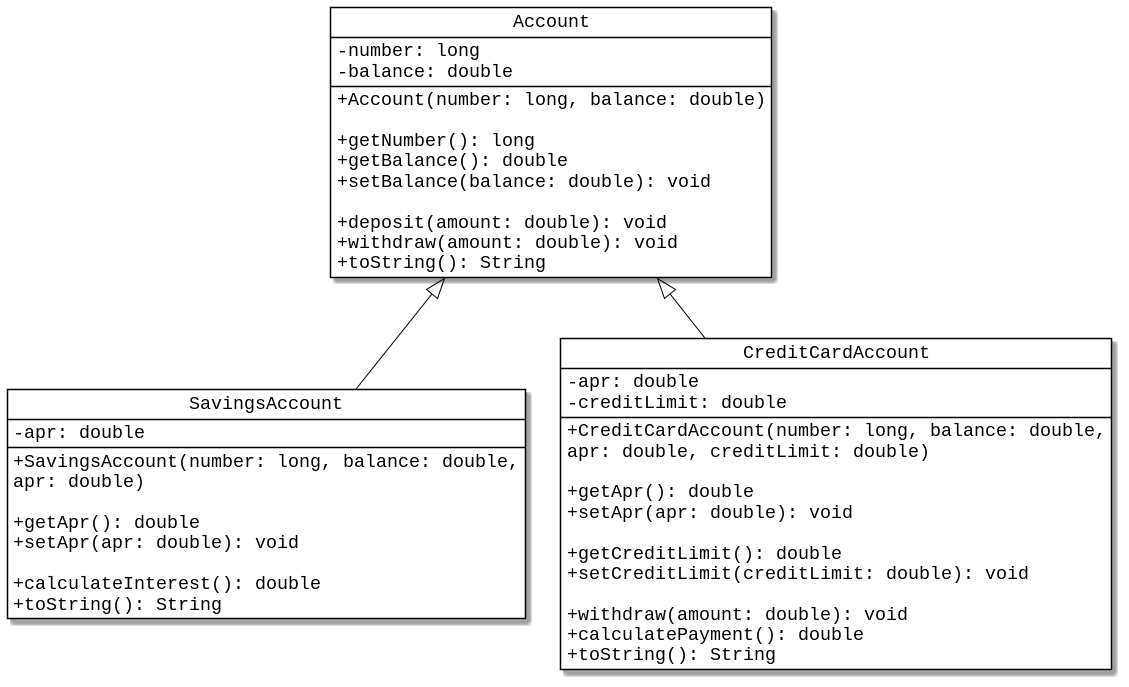
\includegraphics[scale=0.4]{figs/ch14/account_inheritance.png}
\caption{\java{Account}, \java{SavingsAccount}, and \java{CreditCardAccount} classes}
\label{fig.inheritance1}
\end{center}
\end{figure}

\begin{figure}[!ht]
\begin{center}
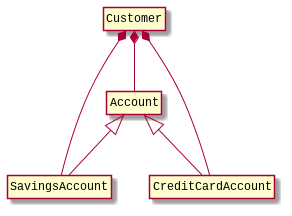
\includegraphics[scale=0.7]{figs/ch14/account_classes.png}
\caption{Composition and Inheritance Among All Classes}
\label{fig.inheritance2}
\end{center}
\end{figure}

{\bf Part 5}: Finally, write a program named {\em TestCustomer.java} that creates a \java{Customer} named ``Joe Doakes'' with this data:

\begin{itemize}
\item Regular account number 1037825 with a balance of \$3,723.00
\item Savings account number 9016632 with a balance of \$4,810.25 and an annual interest rate of 2.05\%
\item Checking account number 85332162 with a balance of -\$2500.00, an interest rate of 7.125\%, and a credit limit of \$3000.00.
\end{itemize}

Then, do the following transactions:

\begin{itemize}
\item Deposit \$257.18 into the regular account, then withdraw \$587.23.
\item Deposit \$2,466.12 into the savings account, then withdraw \$8,000.00.
\item Withdraw \$480.00 from the credit card account.
\item Display the status of the regular account (number and balance).
\item Display the status of the savings account (number, balance, and annual interest amount).
\item Display the status of the credit card account (number, balance, interest rate, and monthly payment due).
\end{itemize}


\end{exercise}

\section{Polymorphism and Dynamic Binding}

Let's return to the \java{Item} and \java{SaleItem} classes.  Try the following program (in the repository in file {\em ch14/Polymorphism.java}) and see what happens:

\begin{code}
public class Polymorphism {
    public static void main(String[] args) {
        Item item1 = new Item("Cat Food", "CF-909", 7.85);
        Item item2 = new SaleItem("Lima Beans", "LB-104",
            5.95, 7.5);
            
        System.out.println("item 1: " + item1.toString());
        System.out.println("item 2: " + item2.toString());
    }
}
\end{code}

The first assignment statement for \java{item1} is no surprise; it assigns an \java{Item} object to an \java{Item} variable. But that second assignment statement---assigning a \java{SaleItem} object to an \java{Item} variable? How can that possibly work? What mad sorcery is this?

\index{polymorphism}
Remember, we're talking about an {\em is-a} relationship. A \java{SaleItem} {\em is an} \java{Item}. That's why it's legal to make the assignment. That is called {\em polyorphism}---the ability to assign a child class object to a parent class variable.

Note that you can't assign a parent object to a child variable. Every \java{SaleItem} is an \java{Item}, but not every \java{Item} is a \java{SaleItem}. If you try this:

\begin{code}
SaleItem badNews = new Item("Oops", "X-000", 6.66);
\end{code}

The compiler will (correctly) complain:

\begin{stdout}
Polymorphism.java:7: error: incompatible types:
  Item cannot be converted to SaleItem
        SaleItem badNews = new Item("Oops", "X-001", 6.66);
\end{stdout}

If you compile and run this program (without the bad line in it), you get this output:

\begin{stdout}
item 1: Cat Food (CF-909): $7.85
item 2: Lima Beans (LB-104): $5.95 - 7.5% discount
\end{stdout}

Take a look at the \java{System.out.println} statements that produced that output. The first one uses \java{Item}'s \java{toString} method to print \java{item1} with its name, SKU, and price.  The second one uses \java{SaleItem}'s \java{toString} method to print \java{item2}'s name, SKU, price {\em and} discount rate.

But both \java{item1} and \java{item2} are \java{Item} objects, so how did the second \java{println} know to call the \java{toString} method from \java{SaleItem}?

\index{dynamic binding}
\index{binding!dynamic}

The answer is {\em dynamic binding}. At compile time, both \java{item1} and \java{item2} have the \java{Item} data type. But at  run time, the JVM looks at the actual object that \java{item2} refers to and finds that it has the \java{SaleItem} data type, and it uses \java{SaleItem}'s \java{toString} method.

This difference between what the compiler sees and what the runtime looks at has very important consequences.

Consider this code, which sets up an array of \java{Item}. Polymorphism allows some of them to be \java{Item} instances and others to be \java{SaleItem} instances:

\begin{code}
public class PolyArray {
    public static void main(String[] args) {
        Item [] foods = {
            new Item("Rye Bread", "RB-010", 3.95),
            new SaleItem("Tomato Soup", "TS-882", 1.29, 0.05),
            new SaleItem("Canned Lima Beans", "CLB-104",
                2.98, 0.155),
            new SaleItem("Frozen Pizza", "FP-326",
                5.90, 0.12),
            new Item("Organic Salsa", "OS-245", 3.79)
        };
// ...
    }
}
\end{code}

We want the program to go through the array and print each item's name and price, and, if it's a sale item, say how much the customer saves:

\begin{stdout}
Rye Bread: $3.95
Tomato Soup: $1.23 - you save $0.06
Canned Lima Beans: $2.52 - you save $0.46
Frozen Pizza: $5.19 - you save $0.71
Organic Salsa: $3.79
\end{stdout}

Here's the pseudo-code for what we want to do:

\begin{code}
for (Item food: foods) {
    System.out.printf("%s: ", food.getName());
    if (food is a sale item) {
        discounted price is getPrice() * (1 - getDiscount());
        amount saved is getPrice() * getDiscount();
        display discounted price and amount saved;
    } else {
        display getPrice();
    }
}
\end{code}

Note that the \java{for} loop variable is an \java{Item}, because we have told the compiler that \java{foods} is an array of \java{Item}.  Here's the big question: how do we determine---at run time---if an array element is a \java{SaleItem} or an \java{Item}? We use the \java{instanceof} operator, which takes the form:

\begin{code}
variable instanceof Class
\end{code}

and returns \java{true} if the given \java{variable} is an instance of \java{Class}; \java{false} otherwise.

A first try at the code looks like this:

\begin{code}
for (Item food: foods) {
    System.out.printf("%s: ", food.getName());
    if (food instanceof SaleItem) {
        double amountSaved = food.getPrice() *
            food.getDiscount();
        System.out.printf("$%.2f - you saved $%.2f\n",
            food.getPrice() - amountSaved, amountSaved);
    } else {
        System.out.printf("$%.2f\n",
            food.getPrice());
    }
}
\end{code}

But when we compile, the compiler tells us:

\begin{stdout}
PolyArray.java:17: error: cannot find symbol
            food.getDiscount();
                ^
  symbol:   method getDiscount()
  location: variable food of type Item
\end{stdout}

Why can't the compiler find \java{getDiscount}? The answer is in {\texttt variable food {\bf of type Item}}. As far as the compiler is concerned, \java{food} is an \java{Item}, and that class does not have a \java{getDiscount} method in it.

What we have to do is use a {\em cast} to tell the compiler, ``yes, we declared it as an \java{Item}, but please treat it as a \java{SaleItem}'':

\begin{code}
for (Item food: foods) {
    System.out.printf("%s: ", food.getName());
    if (food instanceof SaleItem) {
        // tell the compiler to treat food as a SaleItem
        SaleItem saleFood = (SaleItem) food;
        double amountSaved = saleFood.getPrice() *
            saleFood.getDiscount();
        System.out.printf("$%.2f - you saved $%.2f\n",
            saleFood.getPrice() - amountSaved, amountSaved);
    } else {
        System.out.printf("$%.2f\n",
            food.getPrice());
    }
}
\end{code}

Now the compiler is happy---\java{saleFood} is a \java{SaleItem}, and that class has a \java{getDiscount} method.

\section{Summary}


Here's a quick summary of inheritance, polymorphism, and dynamic binding.

\begin{itemize}
\item A subclass (the child class) extends a superclass (the parent class).
\item A subclass constructor can call the superclass constructor by invoking the \java{super} method.
\item If you use a \java{super} constructor, it {\em must} be the first non-comment line.
\item Subclass methods can invoke the superclass methods by using \java{super.method} anywhere in the subclass method body.
\item Polymorphism allows you to assign a subclass object to a superclass variable. For example,

\begin{code}
Item myItem = new SaleItem("Tomato Soup", "TS-882",
   1.29, 0.05);
\end{code}

\item At compile time, the compiler sees the superclass variable as having the superclass data type. In the preceding code, the compiler says that \java{myItem} has data type \java{Item}.

\item At run time, the compiler uses the actual data type of the object. When you say:

\begin{code}
System.out.println(myItem.toString());
\end{code}
    
the JVM will see that \java{myItem} contains a reference to a \java{SaleItem} object and will invoke \java{SaleItem}'s \java{toString} method.
\item The compiler won't let you call a method that exists only in the subclass on a superclass variable. This won't work:

\begin{code}
double saving = myItem.getPrice() * myItem.getDiscount();
\end{code}
    
\java{getPrice} is fine; that method belongs to \java{Item}, but \java{getDiscount} belongs only to the subclass.
\item You can determine if a variable belongs to a class at run time by using the \java{instanceof} operator:

\begin{code}
if (myItem instanceof SaleItem) {
    ...
}
\end{code}
    
\item Once you have established that you have a variable of the subclass data type, you can convince the compiler to treat it as a subclass by using a cast:

\begin{code}
if (myItem instanceof SaleItem) {
    double saving = myItem.getPrice() *
        ((SaleItem) myItem).getDiscount();
}
\end{code}
    
The extra parentheses around the cast are required to get everything evaluated in the correct order.
\end{itemize}

\section{Exercises (concluded)}

\begin{exercise}
This exercise will let you practice polymorphism and dynamic binding. Implement the \java{Bicycle}, \java{ElectricBicycle}, and \java{CargoBicycle} classes. (These are not defined in the same way as in the preceding text.) The parent \java{Bicycle} class has these attributes and methods: 

\begin{itemize}
\item \java{frameSize}, (in centimeters) a double, with a getter (but not a setter).
\item \java{nGears}, an integer, with a getter (but not a setter).
\item \java{currentGear}, an integer, with both a getter and setter.
\item A constructor with two parameters for the frame size and number of gears.
\item A \java{toString} method that includes frame size, number of gears, and current gear, properly labeled.
\end{itemize}

The \java{ElectricBicycle} class is a child of \java{Bicycle} and adds these attributes and methods:

\begin{itemize}
\item \java{batteryCapacity} (in watt-hours), an integer, with a getter (but not a setter).
\item \java{currentCharge} (in watt-hours), a double, with a getter and setter.
\item A constructor with three parameters for frame size, number of gears, and battery capacity.
\item \java{chargePercent}, a method that returns the percentage charge in the battery as a decimal, by dividing current charge by battery capacity.
\item A \java{toString} method that includes frame size, number of gears, current gear, battery capacity, and current charge, properly labeled.
\end{itemize}

The \java{CargoBicycle} class is also a child of \java{Bicycle} and adds these attributes and methods:

\begin{itemize}
\item \java{maxLoad} (in kilograms), a double, with a getter (but not a setter). This is the maximum load that the bicycle can carry.
\item \java{currentLoad} (in kilograms), a double, with a getter and setter.
\item A constructor with three parameters for frame size, number of gears, and maximum cargo load.
\item \java{loadFactor}, a method that returns the percentage of load on the bicycle as a decimal, by dividing the current load by the maximum load.
\item A \java{toString} method that includes frame size, number of gears, current gear, maximum load, and current load, properly labeled.
\end{itemize}

\begin{figure}[!ht]
\begin{center}
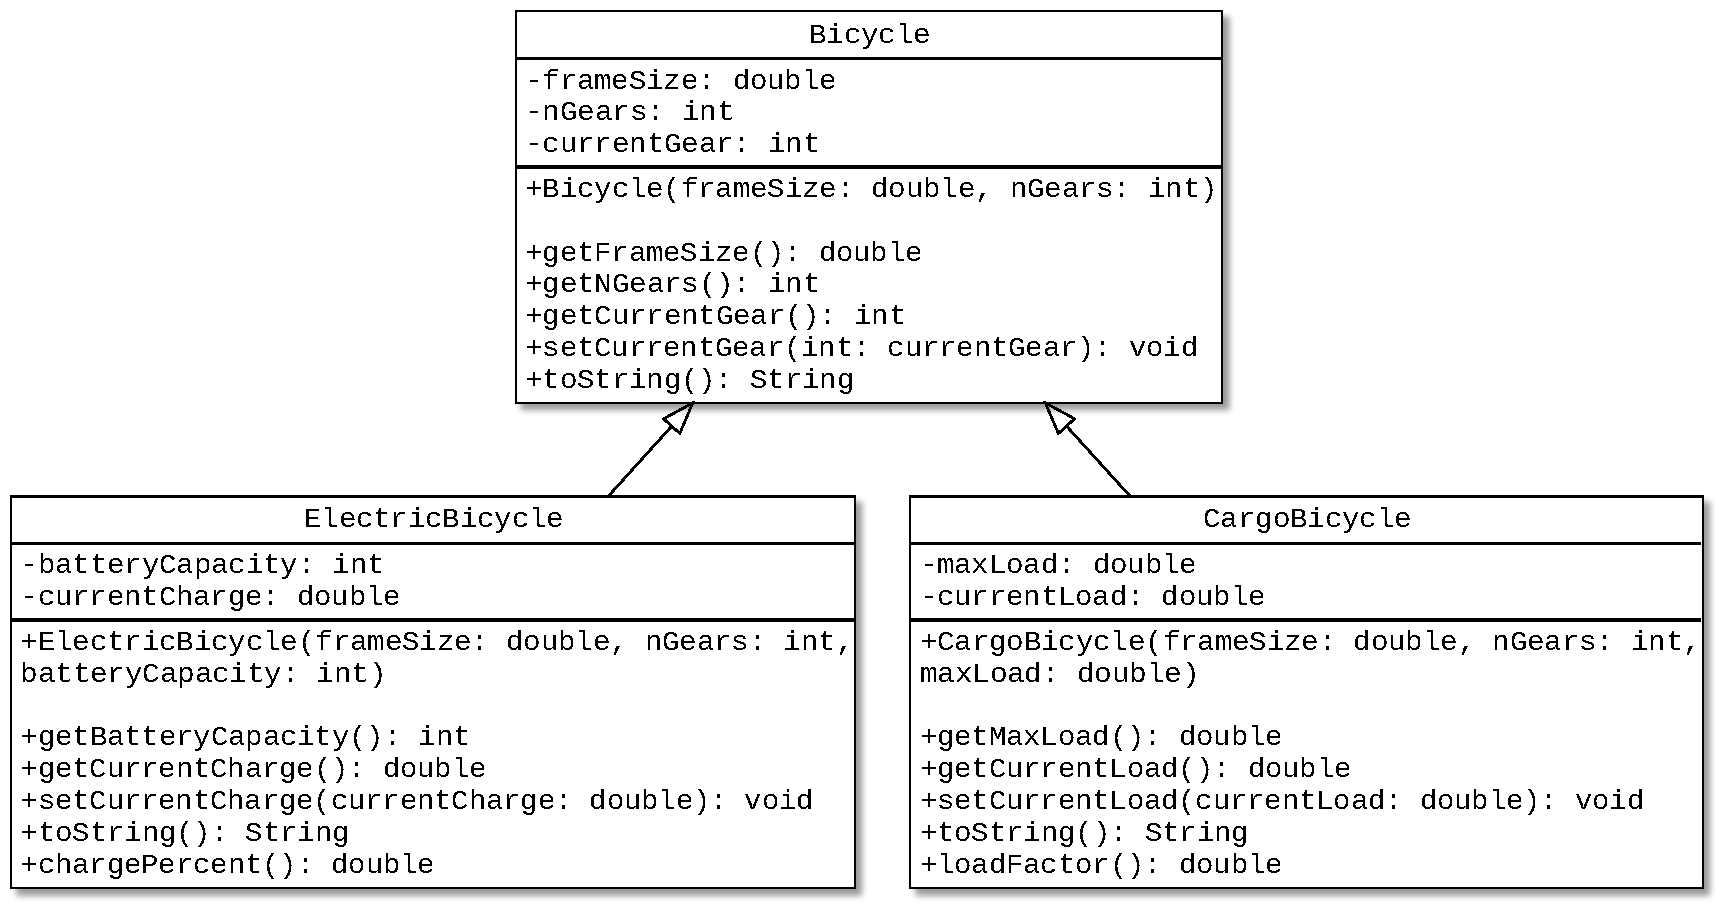
\includegraphics[scale=0.5]{figs/ch14/polymorphism_bikes.pdf}
\caption{UML Diagram of Bicycle, ElectricBicycle, and CargoBicycle}
\label{fig.polyBicycles}
\end{center}
\end{figure}

Figure~\ref{fig.polyBicycles} is the UML diagram for the three classes.

Once you have implemented these classes, write a class named \java{BicycleTest} with a \java{main} method that does the following:

\begin{itemize}
\item Create an array of \java{Bicycle} with these bicycles:
    \begin{itemize}
    \item A bicycle with a 55cm frame, one gear.
    \item An electric bicycle with a 57cm frame, five gears, and a battery capacity of 500 wH (watt-hours).
    \item A cargo bicycle with a 60cm frame, ten gears, and a maximum load of 35kg.
    \end{itemize}
\item Set the electric bicycle's current charge to 312.5 wH.
\item Set the cargo bicycle's current load to 27.5 kg. - note: you may need to use a cast to do this step and the preceding step!
\item Iterate through the array. For each bicycle, call the \java{toString} method and print the information it returns.
    \begin{itemize}
    \item If the entry is an electric bicycle, also print out what percentage charge it has by calling the \java{chargePercent} method and printing its result.
    \item If the entry is a cargo bicycle, also print out what percentage of the maximum load it is carrying by calling the \java{loadFactor} method and printing its result.
    \end{itemize}
\end{itemize}

\end{exercise}

\begin{exercise}
This exercise will let you practice polymorphism and dynamic binding. It uses the \java{Account}, \java{SavingsAccount}, and \java{CreditCardAccount} classes you developed in Exercise~\ref{ex.AccountInheritance}. Instead of creating a customer with multiple accounts, create an array of these accounts:

\begin{itemize}

\item An \java{Account} number 1066 with a balance of \$7,500.
\item A \java{SavingsAccount} number 30507 with a balance of \$4,500 and an APR of 1.5\%
\item A \java{CreditCardAccount} number 51782737 with a balance of \$7,000.00, APR of 8\%, and credit limit of \$1000.00
\item A \java{CreditCardAccount} number 629553328 with a balance of \$1,500.00, an APR of 7.5\%, and a credit limit of \$5,000
\item A \java{CreditCardAccount} number 4977201043L with a balance of -\$5,000.00, an APR of 7\%, and a credit limit of \$10,000 (The \java{L} after the account number lets the compiler know that the account number is a \java{long} integer.)
\end{itemize}

Your program will use a loop to do the following for each account:

\begin{itemize}
\item Deposit \$2,134.00
\item Withdraw \$4,782.00
\item Print the account status using \java{toString()}.
    \begin{itemize}
        \item For savings accounts, also display the annual interest
        \item For credit card accounts, also display the monthly payment
    \end{itemize}
\end{itemize}

Here's what the output might look like:

\begin{stdout}
Account: 1066
Balance: $4852.00

Account: 30507
Balance: $1852.00
Interest Rate: 1.50%
Annual Interest: $27.78

Account: 51782737
Balance: $4352.00
Interest Rate: 8.00%
Credit Limit: $1000.00
Monthly Payment: $0.00

Account: 629553328
Balance: $-1148.00
Interest Rate: 7.50%
Credit Limit: $5000.00
Monthly Payment: $7.18

Account: 4977201043
Balance: $-7648.00
Interest Rate: 7.00%
Credit Limit: $10000.00
Monthly Payment: $20.00
\end{stdout}

\end{exercise}
